\documentclass[twoside,9pt]{report}
\usepackage[a5paper]{geometry}
\usepackage{newpxmath}
%\usepackage{libertine} \usepackage[libertine]{newtxmath}
%\usepackage{kpfonts}
\usepackage{graphicx}
\usepackage{listings}
\usepackage[T1]{fontenc}
\usepackage{imakeidx}
\usepackage{marginnote}
\lstset{
  showstringspaces=false,
  language=tcl,
  frame=lines,
  numbers=left,
  numberstyle=\tiny,
  firstnumber=last,
  basicstyle=\small\ttfamily,
}
%\renewcommand{\thesection}{\arabic{section}}
\title{ConsTcl}
\author{Peter Lewerin}
\date{\today}
\makeatletter
\def\@makechapterhead#1{%
  \vspace*{50\p@}%
    {\parindent \z@ \raggedright \normalfont
      \ifnum \c@secnumdepth >\m@ne
        %\if@mainmatter
          %\huge\bfseries \@chapapp\space \thechapter
          \Huge\bfseries \thechapter.\space%
          %\par\nobreak
          %\vskip 20\p@
        %\fi
      \fi
      \interlinepenalty\@M
      \Huge \bfseries #1\par\nobreak
      \vskip 40\p@
   }}
\makeatother
\makeindex[intoc]
\counterwithout{footnote}{chapter}

\begin{document}
\pagestyle{headings}
\maketitle
\tableofcontents

\chapter{Introduction}
\label{introduction}
\section{To run the software}
\label{to-run-the-software}
\index{to run the software}


First things first. To run, source the file \textbf{constcl.tcl} (with
\textbf{schemebase.lsp} in the directory) in a Tcl console (I use
\textbf{tkcon}) and use the command \textbf{repl} for a primitive command
dialog. Source \textbf{all.tcl} to run the test suite (you need
\textbf{constcl.test} for that). The files can be found on GitHub/ConsTcl\footnote{See
\texttt{https://github.com/hoodiecrow/ConsTcl}}.

\section{Background}
\label{background}
\index{background}

It all started with Peter Norvig's Lisp emulator
Lispy\footnote{See \texttt{https://norvig.com/lispy.html}}. In January 2025 I
was inspired to port it to Tcl. The result was Thtcl\footnote{See
\texttt{https://github.com/hoodiecrow/thtcl}}. It had the same features and
limitations as Lispy, plus a couple that were due to shortcomings of Tcl, and I
came out of the experience feeling a bit dissatisfied. In the latter part of
January I embarked on a new project, ConsTcl, a true Lisp interpreter. In Tcl.

\subsubsection{About ConsTcl}
\label{about-constcl}

It's written with Vim, my editor of choice. I'm using annotated source which
mixes code with documentation and test cases. Compared to Lispy/Thtcl, ConsTcl
has, quote from Lispy, comments, quote and quasiquote notation, \# literals,
the derived expression types (such as cond, derived from if, or let, derived
from lambda), and dotted list notation. And also real consed lists. Again
compared to Lispy/Thtcl, ConsTcl has the data types, quote, strings,
characters, booleans, ports, vectors. And pairs and procedures too. The number
of missing primitive procedures is in the tens, not the 100s. The completeness
comes with a price: due to the sheer number of calls for each action, ConsTcl
is is fairly slow. On my cheap computer, the following code (which calculates
the factorial of 100) takes 0.03 seconds to run. That is ten times slower than
Lispy assuming that Norvig's computer is as slow as mine, which is unlikely.

\begin{verbatim}
time {pe "(fact 100)"} 10
\end{verbatim}

ConsTcl is of course still limited. It doesn't come close to having call/cc or
tail recursion. It doesn't have exact/inexact numbers, or most of the numerical
tower. There is no memory management. Error reporting is spotty, and there is no
error recovery.

\subsubsection{About the book}
\label{about-the-book}


I like writing documentation, and occasionally I'm good at it. I like to
annotate the source code with bits of documentation, which I then extract and
put together using tools like \texttt{awk}. It looks like this:

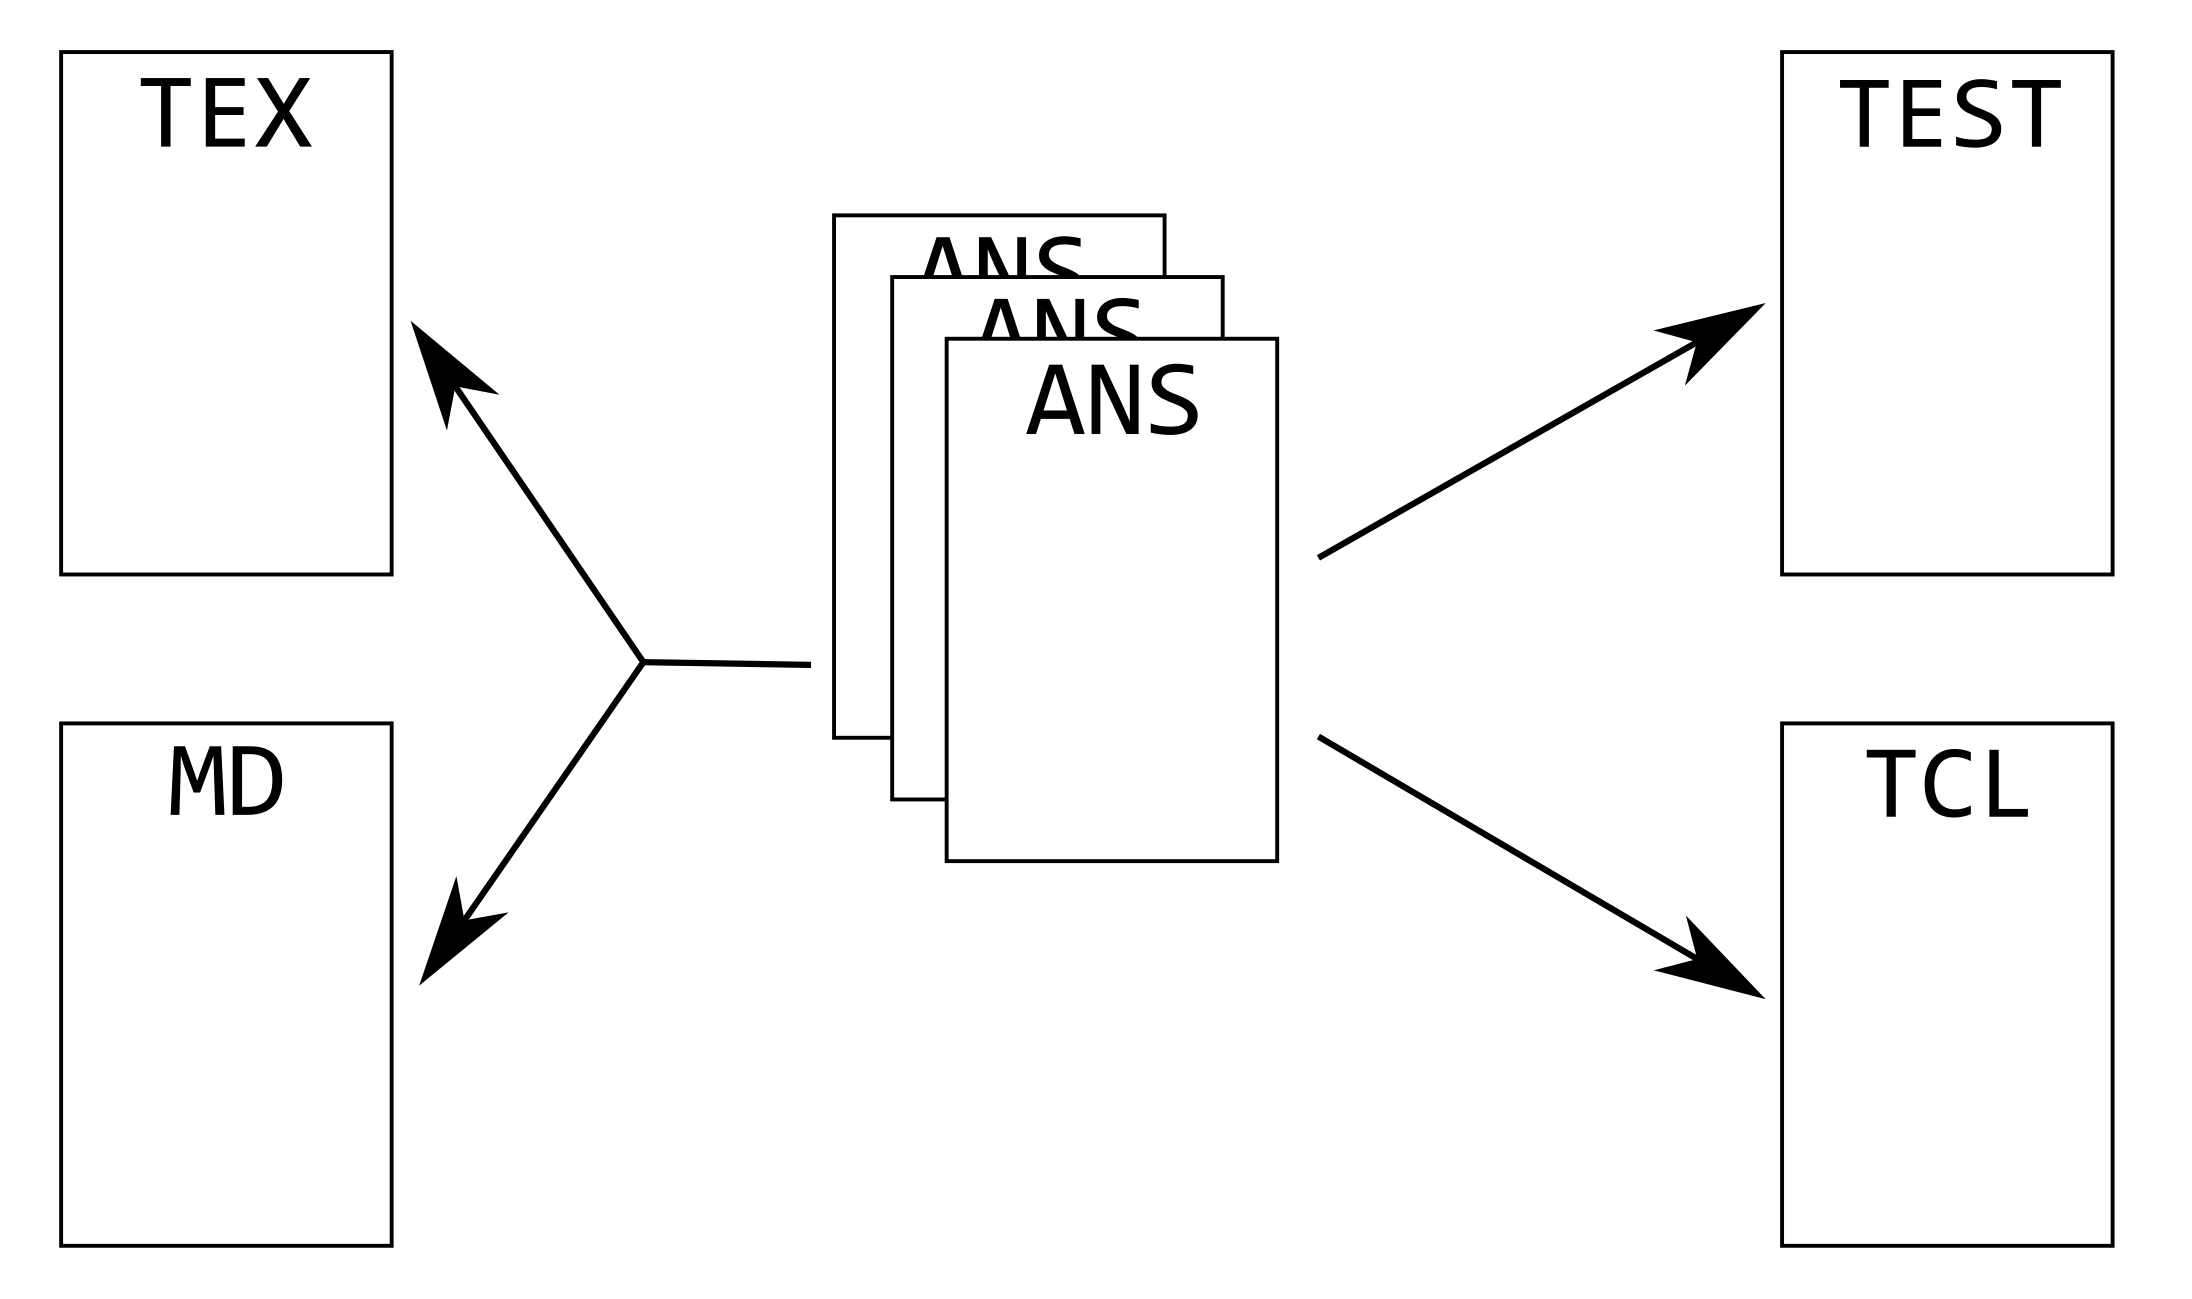
\includegraphics{images/document.png}

In the middle are a bunch of \texttt{.ans} files (ANnotated Source). From the
TT tags of those, I extract a \texttt{.test} file. From the CB tags I extract
\texttt{.tcl} source. From all the tags except TT I extract formatted
documentation in Markdown and (La)TeX format. All these extractions are
automated using \texttt{make}. I create a PDF document from the (La)TeX source
using TeXworks. On finishing up ConsTcl, it struck me that the documentation
for this piece of software was fit for a book.

\subsubsection{About the program listings}
\label{about-the-program-listings}


I have tried to write clear, readable code, but the page format forces me to
shorten lines. I have used two-space indents instead of four-space, a smaller
font, and broken off long lines with a \textbackslash\  at the end of the first
line (a so-called "tucked-in tail"). Neither of these measures improve
readability, but the alternative is overwriting the margins. Not all broken
lines have the \textbackslash: some are broken inside a
\texttt{\{}\ldots\texttt{\}} block, and some right after a \texttt{[}.

\subsubsection{About me}
\label{about-me}

I'm a 60 year old former system manager who has been active in programming
since 1979. Currently, since around 25 years, my language of choice is the
rather marginal Tcl (it's not even in the 100 most used languages). Tcl suits
me, and there are things that one can do in Tcl that one can't easily do in
other languages. Lisp is a runner-up in my affections, a language that
fascinates me but doesn't fit my brain very well (though I have written one
large piece of software in AutoLisp, a CAD subsystem for designing drilling
equipment).

In addition to my terms as programmer and system manager, I have worked as a
teacher (teaching C/C++ in upper secondary school) and for a short while I
produced textbooks for the department for information technology at
the University of Skövde. I've also been active writing answers at
question-and-answer sites on the web, mainly Stack Overflow.

